\documentclass{article}

\usepackage[margin=1.6cm]{geometry}
\usepackage{amsmath,amssymb}
\usepackage{float}
\usepackage{graphicx}
\usepackage{fancyhdr}
\pagestyle{fancy}
\usepackage{tcolorbox,listings}
\usepackage{color}
\usepackage{hyperref}
\renewcommand\headrulewidth{1pt}
\usepackage{marvosym}
\usepackage{xcolor}
\usepackage{tikz}
%\usepackage{babel}
\usepackage[french]{babel}
\usepackage[babel=true,kerning=true]{microtype}
\usepackage{afterpage}

\newcommand\myemptypage{
    \null
    \thispagestyle{empty}
    \addtocounter{page}{-1}
    \newpage
    }

\usetikzlibrary{
  arrows,
  calc,
  shapes.geometric,
  shapes.misc,
  shapes.symbols,
  shapes.arrows,
  automata,
  through,
  positioning,
  scopes,
  decorations.shapes,
  decorations.text,
  decorations.pathmorphing,
  shadows}

\definecolor{darkWhite}{rgb}{0.94,0.94,0.94}
 
\lstset{
    backgroundcolor=\color{darkWhite},
    breakatwhitespace=false,
    breaklines=true,
    captionpos=b,
    commentstyle=\color{green},
    deletekeywords={...},
    escapeinside={\%*}{*)},
    extendedchars=true,
    keepspaces=true,
    keywordstyle=\color{blue},
    %language=Python,
    morekeywords={*,...},
    showspaces=false,
    showstringspaces=false,
    showtabs=false,
    stepnumber=1,
    stringstyle=\color{gray},
    tabsize=4,
}
 
\lstdefinestyle{frameStyle}{
    basicstyle=\sffamily,
    numbers=left,
    numbersep=20pt,
    numberstyle=\tiny\color{black}
}
 
\tcbuselibrary{listings,skins,breakable}
 
\newtcblisting{customFrame}{
    arc=0mm,
    top=0mm,
    bottom=0mm,
    left=3mm,
    right=0mm,
    width=\textwidth,
    listing only,
    listing options={style=frameStyle},
    breakable
}

\fancyhead[L]{ALLEMAND Fabien\\??? Samuel}
\fancyhead[C]{Compilation}
\fancyhead[R]{
\includegraphics[scale=0.08]{img/logo_UFR_1.png}}
\fancyfoot[L]{Rapport de Projet}
\fancyfoot[R]{\today}

\begin{document}

\newpage
\thispagestyle{empty}
\addtocounter{page}{-1}
\begin{center}
	\baselineskip=50pt
	\vspace*{1cm}
	\textbf{{\Huge Compilation}}\\
	\vspace*{0.25cm}
	\textbf{{\Huge Rapport de Projet}}\\
	\vspace*{0.25cm}
	\begin{minipage}[c]{.46\linewidth}
        \centering
        \textbf{Equipe:}\\
		ALLEMAND Fabien\\
        ??? Samuel
    \end{minipage}
\end{center}
\vspace{0.1cm}

\begin{figure}[H]
\centering
\centerline{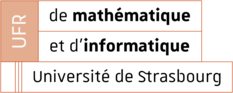
\includegraphics[scale=1.]{img/logo_UFR_2.png}}
\end{figure}

\newpage
\myemptypage

% \pagenumbering{roman}

% \newpage
% \myemptypage

\newpage
% \addcontentsline{toc}{section}{Table des matières}
\renewcommand{\contentsname}{Table des matières}
\tableofcontents

\newpage
\addcontentsline{toc}{section}{Liste des figures}
\renewcommand{\listfigurename}{Liste des figures}
\listoffigures

\pagenumbering{arabic}

\newpage
\section{Introduction}

\paragraph{}
La compilation consiste à traduire un code source lisible par un humain en un code exécutable par un ordinateur. C'est à dire transformer un fichier texte contenant des instructions écrites dans un langage de programmation en un fichier binaire.

\paragraph{}
Ce projet consiste à écrire un compilateur pour un langage de programmation impératif simple appelé SoS qui utilise une syntaxe et des fonctionnalités issues d'un sous-ensemble de langage shell
unix (Sous-Shell).\\
\'Ecrit en C et en utilisant les outils \textsf{Flex} et \textsf{Bison}, le compilateur est capable de traduire un programme écrit en SoS en une suite d'instructions MIPS pouvant être exécutées à l'aide d'un simulateur.

\paragraph{}
Dépôt Git: \url{https://github.com/FABallemand/ProjetCompilation}

\newpage
\section{Conclusion}

\paragraph{}
Le compilateur que nous avons écrit (bien qu'assez peu performant) permet de compiler correctement des programmes écrits dans le langage SoS.\\
L'analyseur lexical et l'analyseur syntaxique permettent de générer du code intermédiaire. Nous avons accordé une attention particulière à la table de symboles et à la gestion des contextes.\\
La traduction en code MIPS est assurée par un programme en C qui traduit le code intermédiaire en MIPS et une bibliotèque de fonctions MIPS.

\paragraph{}
La compilation est encore de nos jours un domaine de recherche en plein essor. De nouvelles contraintes liées à la performance mais aussi à l'efficacité énergétique du code généré donnent lieu à de nouvelles méthodes d'optimisation parfois très complexes.\\
Cet aspect de la compilation n'a malheureusment pas pu être abordée lors de ce projet. Sans doute de nombreuses améliorations peuvent être apportées à ce compilateur!

\newpage
\addcontentsline{toc}{section}{Bibliographie}
\renewcommand{\refname}{Bibliographie}
\bibliographystyle{plain}
\bibliography{bibliographie}

\newpage
\myemptypage

\newpage
\input{src/annexes.tex}

\end{document}